\documentclass[conference]{IEEEtran}

%XXX Remove before final submission
\usepackage{todonotes}
\usepackage{cite}
\usepackage{amsmath}
\usepackage{caption}
\usepackage{subcaption}
\usepackage{subcaption}
\usepackage[linesnumbered,ruled,vlined]{algorithm2e}
% Note that the amsmath package sets \interdisplaylinepenalty to 10000
% thus preventing page breaks from occurring within multiline equations. Use:
%\interdisplaylinepenalty=2500
% after loading amsmath to restore such page breaks as IEEEtran.cls normally
\usepackage{url}
\usepackage{hyperref}
\usepackage{verbatim}
\usepackage{siunitx}
\usepackage{listings}
\usepackage{mathtools}
\DeclarePairedDelimiter\ceil{\lceil}{\rceil}
\DeclarePairedDelimiter\floor{\lfloor}{\rfloor}


\lstdefinelanguage{Julia}{
  basicstyle=\small\ttfamily,
  showspaces=false,
  showstringspaces=false,
  keywordstyle={\textbf},
  morekeywords={if,else,elseif,while,for,begin,end,quote,try,catch,return,local,abstract,function,stagedfunction,macro,ccall,finally,typealias,break,continue,type,global,module,using,import,export,const,let,bitstype,do,in,baremodule,importall,immutable},
  escapeinside={~}{~},
  morecomment=[l]{\#},
%  commentstyle=\textsf,
  commentstyle={},
  morestring=[b]",
}

\lstset{language=Julia,basicstyle=\footnotesize\ttfamily,breaklines=true}

% correct bad hyphenation here
\hyphenation{}


\begin{document}

%XXX remove before submission
\newcommand{\TODO}[1]{\todo[inline]{#1}}
\newcommand{\TODOFIG}[1]{\missingfigure{#1}}

\title{Catchy Title Here}

% author names and affiliations
% use a multiple column layout for up to three different
% affiliations
\author{\IEEEauthorblockN{Jiahao Chen and Jarrett Revels}
\IEEEauthorblockA{Computer Science and Artificial Intelligence Laboratory\\
Massachusetts Institute of Technology\\
Cambridge, Massachusetts 02139--4307\\
Email: \{jiahao,jrevels\}@csail.mit.edu}
}

% make the title area
\maketitle

%%%%%%%%%%%%%%%%%%%%%%%%%%%%%%%%%%%%%%%%%%%%%%%%%%%%%%%%%%%%%%%%%%%%%%%%%%%%%%%%%%%%%%%%%%%%
\begin{abstract}
We propose a rigorous methodology for automated benchmarking and regression detection in the
presence of timer error, OS jitter and other environmental fluctuations. By examining data
obtained from Julia benchmarks, we demonstrate the ways in which timing distributions can
violate many of the statistical assumptions made by other benchmarking frameworks. From our
experimental observations, we construct a model and an accompanying benchmarking
strategy which purposefully avoids these assumptions. This strategy makes efficient use of
user time constraints by simultaneously maximizing the number of measurements per trial
while minimizing inter-measurement timing variations, rendering it suitable for continuous
integration (CI) pipelines, even when applied to relatively large benchmark suites. Using
our model, we formulate a robust, nonparametric hypothesis test that makes use of the
subsampling method to estimate the statistical significance of observed variations
in execution time. We test our methodology on a small collection of mock Julia benchmarks,
discussing where it succeeds relative to other methods as well as pointing out potential
pitfalls. Finally, we discuss a prototype implementation of the proposed method that was
recently released to aid in the development of the Julia language and ecosystem, which has
already caught and prevented several performance regressions in Julia's base library.
\end{abstract}

\IEEEpeerreviewmaketitle

\TODO{come up with better section/subsection names}

%%%%%%%%%%%%%%%%%%%%%%%%%%%%%%%%%%%%%%%%%%%%%%%%%%%%%%%%%%%%%%%%%%%%%%%%%%%%%%%%%%%%%%%%%%%%
\label{sec:intro}
\section{Introduction}

Developers of high performance applications often rely on benchmark suites to determine the
impact of code changes on program performance. Despite the importance of these suites in
safeguarding against performance regressions, developers often run and interpret them in an
ad hoc manner. This disregard for proper experimental methodology wastes development time
and may lead to misguided decisions that worsen performance.

In this paper, we consider the problem of designing a language- and platform-agnostic
benchmarking methodology for rigorously testing large benchmark suites within reasonable
time constraints, rendering it suitable for continuous integration (CI) pipelines and manual
user workflows. Our goal is to define an experimental protocol and a statistical test for
automatically and reproducibly detecting performance regressions with respect to a given
benchmark suite, quantifying detection confidence using rigorous estimates of statistical
significance.

In practice, the complexity of modern hardware and software enviroments reduces the
reliability of regression detection frameworks by introducing undesirable variations in
timing measurements and application performance. System quiescence research has acknowledged
that these variations induce non-Gaussianity in performance statistics. Despite this
research, current statistical approaches to regression detection improperly assume the
Gaussianity of timing measurement distributions. We present a statistical model that, in
contrast, provides an explicitly non-Gaussian formulation of timing variations. We
substantiate our model using data obtained from a small set of mock Julia benchmarks.

\label{sec:timererror}
\paragraph{The effects of timer measurement error}

Our methodology pays special attention to benchmarks whose expected execution time is on the
order of 1 microsecond or shorter, which is quick enough that the benchmark is vulnerable to
error due to insufficient system timer accuracy on modern platforms. A common technique for
accurately measuring the runtime of these benchmarks is to time multiple executions of the
benchmark, estimating the runtime of a single execution by dividing the measured time by the
number of executions.

\TODO{Cite strategies for orchestrating performance counters}

\label{sec:environment}
\paragraph{Controlling for environmental effects}
Modern hardware and operating systems introduce many confounding factors that
complicate a developer's ability to reason about variations in user-space
application performance~\cite{HP5e}.

At the hardware level, changes in temperature, workload, and power availability
can trigger CPU clock frequency scaling to limit power consumption.
External factors such a high network traffic may also trigger interrupts at the
OS level.
At the operating system level, sources of variation are often referred to as
OS jitter.
Jitter may be caused by randomizing security features like address space layout
randomization (ASLR)~\cite{Shacham2004},
virtual memory management~\cite{Oyama2014,Oyama2016},
changing between CPU privilege levels like kernel mode and user mode~\cite{Zaparanuks2009},
context switching overhead to handle interrupts~\cite{Tsafrir2007},
activity from system daemons and cluster managers~\cite{Petrini2003},
or even suboptimal process- and thread-level scheduling~\cite{Lozi2016}.
Even seemingly irrelevant configuration parameters like the size of the
OS environment can confound reproducibility. Changing the size of the
environment moves the call stack, which is loaded after the environment, which
in turn changes the alignment of data in memory~\cite{Mytkowicz2009}.

The choice of programming language compiler parameters can result in yet
further timing variations.
Compiler optimizations can adversely affect the accuracy of hardware
counters~\cite{Zaparanuks2009}, or in extreme cases eliminate key parts of the
microbenchmark as dead code.
For compiled languages, the linker is free to choose the binary layout of the
library or executable arbitrarily, resulting in nondeterministic memory
layouts~\cite{Georges2008}. This problem is exacerbated in languages like C++,
whose compilers introduce random name mangling of symbols~\cite{Kalibera2005}.
Additionally, the behavior of the runtime can change depending on OS or hardware
parameters. For example, changing the heap size can affect garbage collector
performance~\cite{Blackburn2004}.

Most of these studies focus on Java programming language and/or the Linux OS.
While the phenomena described clearly apply to general software and hardware environments,
mitigating strategies are often highly specialized, ranging from custom OS
kernels \cite{Tessellation,Akkan2012}, custom compilers providing
reproducible~\cite{Georges2008} or consistently randomized~\cite{Curtsinger2013}
binary layouts, to low-variability garbage collectors~\cite{Huang2004}.
These mechanisms for achieving quiescence are platform dependent, deviate strongly
from a typical user's machine and configuration, or cannot be reasonably automated without
root access to the user's machine. Reliance on these techniques could negatively impact
portability and thus decrease the likelihood of adoption.

\TODO{cite/discuss Kalibera's paper on ``benchmarking in reasonable time'', and similar
papers}

\label{sec:stats}
\subsection{Doing stastistics on timing measurements is hard}

The myraid sources of environmental variation must all be mitigated against to
produce a reproducible state in which to run the benchmark program. In practice,
it is impossible to eliminate variation entirely~\cite{Alcocer2015,Barrett2016}.
Therefore, software for microbenchmarking must account for both measurement error
and environmental factors of variation.
One approach taken by microbenchmarking packages like Haskell's
\lstinline|criterion|~\cite{criterion} collects multiple timing measurements
with increasing number of benchmark executions, which are used to estimate the
run time as the gradient of the ordinary least squares regression line.
However, the least squares fit is sensitive to outliers (which are detected and
reported by \lstinline|criterion|), and requires many evaluations of the benchmark.
Furthermore, many of the shorter timing measurements are contaminated by timer
inaccuracy, which contributes to the error in estimating the true benchmark run time.
One approach based on variance reduction requires strong assumptions on the
underlying statistics, such as the existence of fourth moments and the lack of
large outliers~\cite{Kalibera2006,Kalibera2013}.

\begin{figure}
\centering
\begin{subfigure}{0.22\textwidth}
    \centering
    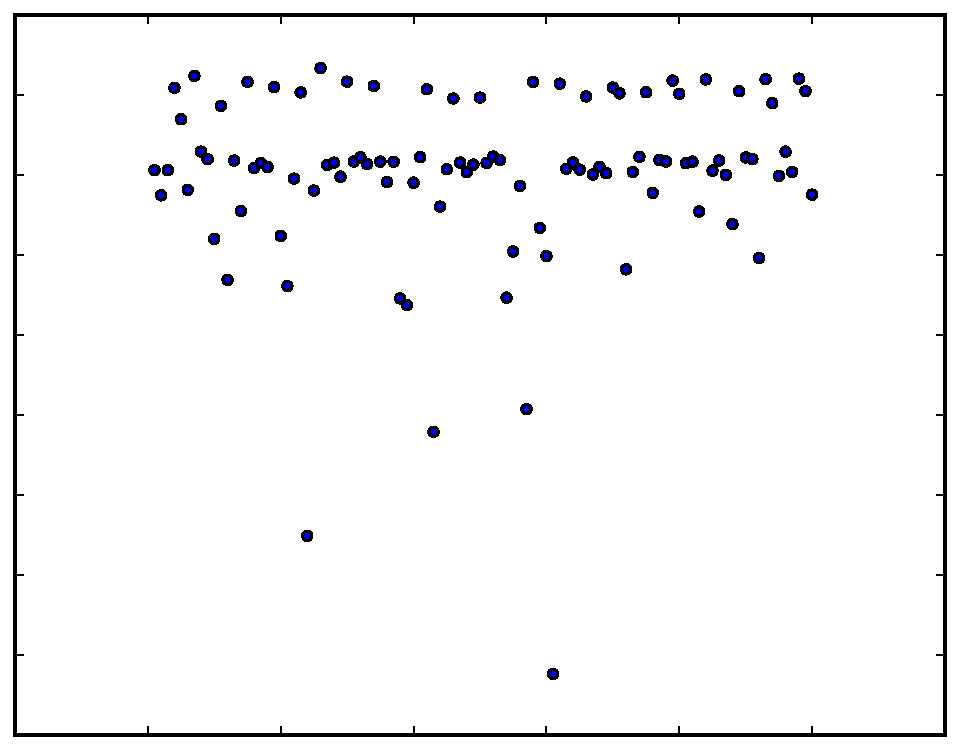
\includegraphics[width=\textwidth]{figures/fig1/simple_branchsum_fast}
    \caption{Benchmark 1: Unimodal with skew and large outliers}
\end{subfigure}%
~
\begin{subfigure}{0.22\textwidth}
    \centering
    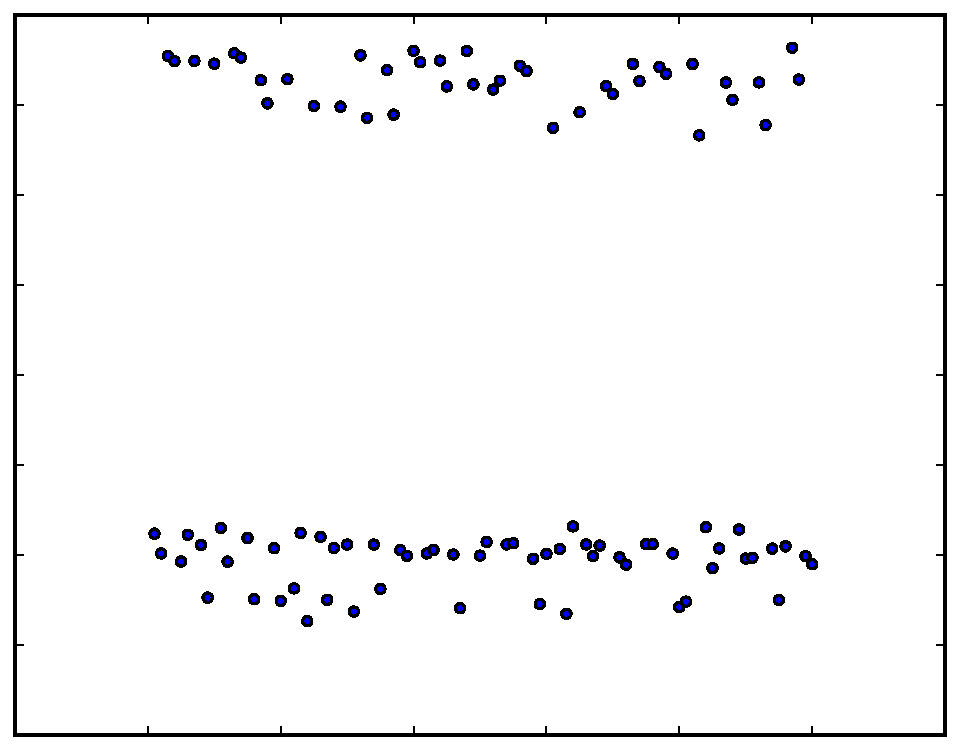
\includegraphics[width=\textwidth]{figures/fig1/bimodal_branchsum}
    \caption{Benchmark 2: Bimodal}
\end{subfigure}
\begin{subfigure}{0.22\textwidth}
    \centering
    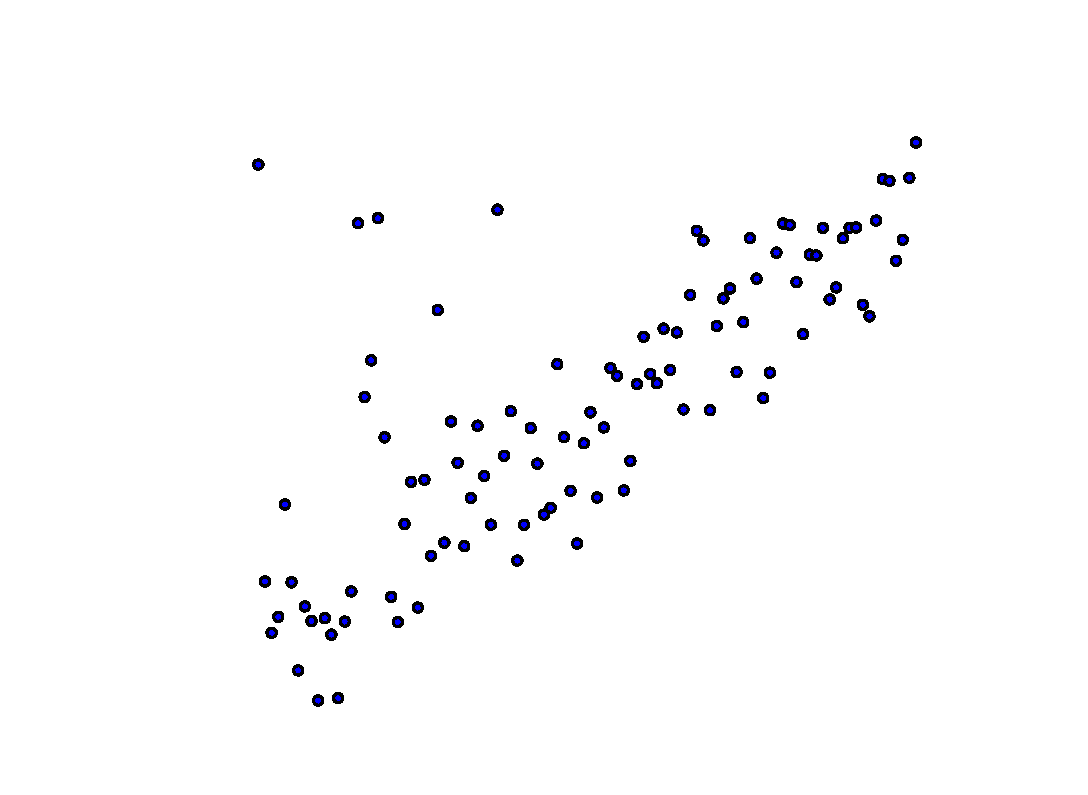
\includegraphics[width=\textwidth]{figures/fig1/drift_manyallocs_slow}
    \caption{Benchmark 3: Drift}
\end{subfigure}
~
\begin{subfigure}{0.22\textwidth}
    \centering
    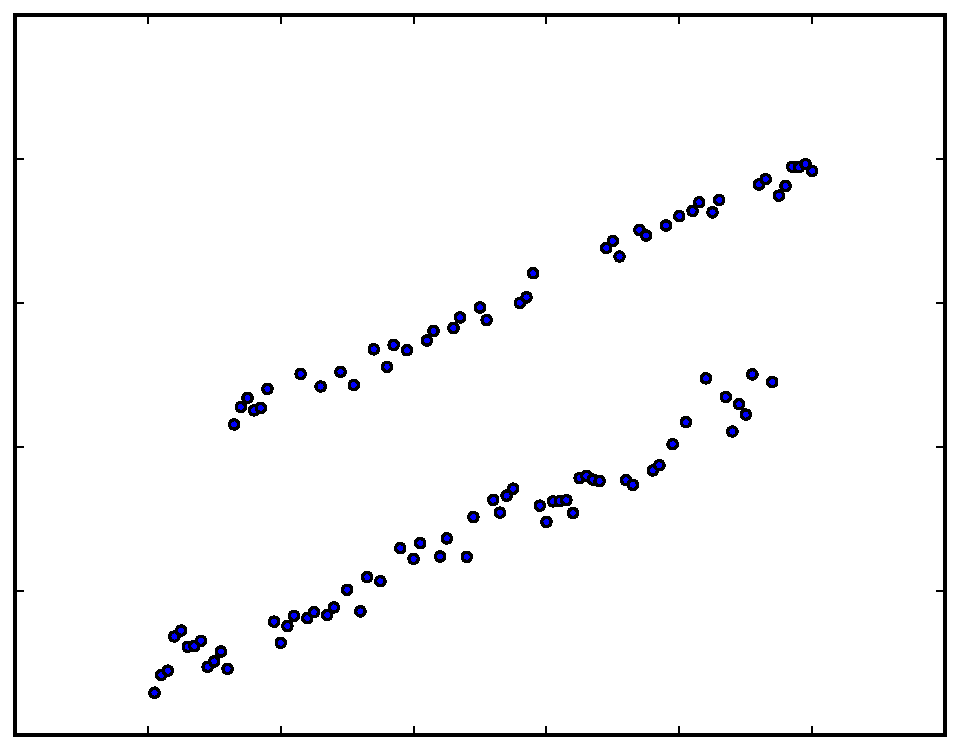
\includegraphics[width=\textwidth]{figures/fig1/bimodal_drift_sumindex}
    \caption{Benchmark 4: Bimodal with drift}
\end{subfigure}
\caption{Variability in the mean benchmark time across multiple trials, showing
that the mean has non-iid, nonnormal behavior in four different benchmarks.
Each point represents a mean time computed from trial of 10,000 measurements.
The horizontal axis is the index of the trial, while the vertical axis is time.}
\label{fig:meandistributions}
\end{figure}

Benchmark times usually do \textit{not} exhibit iid normal statistics,
which are assumed in textbook comparisons using $t$-tests or
$F$-ratios~\cite{Lilja2000} and in some benchmarking programs like AndroBench,
which use a 3-sigma rule for defining outliers.
Contrary to these standard assumptions,
we see a wide variety of statistical behaviors in actual measurements;
Figure~\ref{fig:meandistributions} shows that even for the four illustrative
benchmarks considered in this paper, none of them show iid normal behavior.
The first benchmark exhibits a skewed density and has many outliers on one side.
The second benchmark has a bimodal distribution.
The third benchmark shows a consistent drift, with the measured time increasing
as the benchmark trial is rerun.
The fourth benchmark shows a complicated distribution exhibiting bimodality and
drift.
Such nonideal statistics have also been observed in other
studies~\cite{Gil2011,Chen2015,Rehn2015,Barrett2016}.
In these situations, the standard tests have poor statistical
power~\cite{Mytkowicz2009,Kalibera2013,Chen2015,Barrett2016}.
Other authors have suggested removing outliers to improve
Gaussianity~\cite{Rehn2015}\TODO{and loc. cit.}, but these methods would
qualitatively alter the statistics shown in our exemplar benchmarks.
A better approach is to use robust statistics such as the median as a location
parameter~\cite{Hampel1971,Mytkowicz2009,Touati2013}.
However, we will argue in the next section that the minimum is a more appropriate
location parameter for regression benchmarking.

%%%%%%%%%%%%%%%%%%%%%%%%%%%%%%%%%%%%%%%%%%%%%%%%%%%%%%%%%%%%%%%%%%%%%%%%%%%%%%%%%%%%%%%%%%%%
\label{sec:notation}
\section{Notation}

The rest of this paper utilizes a consistent notation for discussing various statistical and
measured quantities related to benchmarking. We define this notation here:

\begin{itemize}
    \item
    $P_0$, $P$ and $Q$ denote \textbf{benchmarkable programs}, each defined by a tape of
    instructions.

    \item
    $I^{[i]}_{P}$ is the $i^{\textrm{th}}$ \textbf{instruction} in the tape defining program $P$.
    Instruction indices are always written using bracketed superscripts, $\cdot^{[i]}$.

    \item
    $D^{[i]}_{P}$ is the \textbf{delay instruction} associated with $I^{[i]}_{P}$. Delay
    instructions are precisely defined in Section~\ref{sec:model}.

    \item
    $T_i$ is a \textbf{timing measurement}. Specifically, $T_i$ is the amount of time taken
    to perform $n_i$ \textbf{executions} of a benchmarkable program. This quantity is
    directly measurable via experiment.

    \item
    $t$ is an \textbf{execution time}. Specifically, $t$ is the amount of time it takes to
    perform a single execution of a benchmarkable program. This quantity is not generally
    measured directly but is instead derived as $t_i = T_i / n_i$.

    \item
    \textbf{Estimated quantities} are denoted with a hat, $\hat\cdot$. For example,
    $\hat{t}_{\textrm{min}}$ is the estimated value for the minimum value of the benchmark execution
    time.

    \item
    \textbf{Resampled quantities} are denoted with a superscript asterisk, $\cdot^*$. For
    example, $t^*_1, \dots t^*_m$ is a resample of $t_1, \dots t_n$.

    \item
    A benchmark \textbf{experiment} is a recipe for obtaining multiple timing measurements
    for a benchmarkable program. Experiments can be executed to obtain \textbf{trials}. The
    $i^{\textrm{th}}$ trial of an experiment is a collection of timing measurements
    $T^{\{i\}}_1, \dots T^{\{i\}}_j, \dots T^{\{i\}}_k$. Trial indices are always
    written using embraced superscripts, $\cdot^{\{i\}}$.

    \item
    $\tau$ denotes time quantities that are external to the benchmarkable program:
    \begin{itemize}
        \item $\tau_{\textrm{budget}}$ is the \textbf{time budget} for an experiment.
        \item $\tau_{\textrm{acc}}$ is the \textbf{accuracy} of the system timer.
        \item $\tau_{\textrm{prec}}$ is the \textbf{precision} of the system timer.
    \end{itemize}

    \item
    $\epsilon^{(i)[j]} = x_P^{(i)[j]} \tau^{(i)}$ is the \textbf{time delay} due to the
    $i^{\textrm{th}}$ \textbf{delay factor} for delay instruction $D^{[j]}$.  Specifically,
    $\tau^{(i)}$ is the factor's \textbf{time scale} and $x_P^{(i)[j]}$ is the factor's
    \textbf{trigger coefficient} for $D^{[j]}$. Delay factor indices are written using
    parenthesized superscripts, $\cdot^{(i)}$.

    \item
    $E_P^{(i)}$ is the total \textbf{cumulative delay} due to the $i^{\textrm{th}}$ delay
    factor during the execution of program $P$.

    \item
    $X^{(i)}_P$ is the total \textbf{cumulative trigger count} of the $i^{\textrm{th}}$
    delay factor during the execution of program $P$.

    \item
    $\nu(t)$ is an \textbf{oracle function} that, given an execution time $t_P$, estimates
    an appropriate $n_P$ necessary to overcome measurement error due to insufficient
    $\tau_{\textrm{acc}}$ and $\tau_{\textrm{prec}}$.

    \item
    $f_X(\xi)$ is the \textbf{probability density function (pdf)} associated with the random
    variable $X$. $\int_{x}^{x+\delta x} f_X(\xi) d\xi$ is the probability that $x < X <
    x+\delta x$.
\end{itemize}

%%%%%%%%%%%%%%%%%%%%%%%%%%%%%%%%%%%%%%%%%%%%%%%%%%%%%%%%%%%%%%%%%%%%%%%%%%%%%%%%%%%%%%%%%%%%
\label{sec:model}
\section{A better statistical interpretation of benchmark timing distributions}

In this section, we present a statistical description of benchmark behavior that avoids
problematic assumptions of normality or identical timing distributions between benchmarks.
This model will drive the design of the experimental protocol and the hypothesis test
that we discuss in future sections.

\subsection{The underlying model for program execution}

Consider an initial benchmarkable user program $P_0$, whose output is deterministic and
identical for every execution of the program. $P_0$ can be specified by as a sequence of
instructions $I^{[i]}$:

\begin{equation}
    P_0 = \left[I^{[1]}, I^{[2]}, \dots I^{[k]}\right]
\end{equation}

Each instruction $I^{[i]}$ specifies a state transition that takes the executing machine
from an initial state to a desired output state. In an idealized universe, we could assume
that the state transition for instruction $I^{[i]}$ takes exactly $\tau^{[i]}$ time, such
that the total runtime of $P_0$ is $t_{P_0} = \sum_{i=1}^N \tau^{[i]}$.

In reality, the machine and operating system executing $P_0$ are vulnerable to the factors
described in Section~\ref{sec:challenges}. These factors may cause the computer to undergo
zero or more intermediary state transitions before achieving the state transistion specified
by instruction $I^{[i]}$. Since these factors \textit{delay} the completion of the original
instructions, we refer to them as \textit{delay factors}\footnote{Technically, there are
some causes of timing variations which might speed up the execution of a program, such as
frequent scaling \TODO{cite}. However, these factors number far fewer than those that slow
down execution of a program, and as such, are more easily controlled. Thus, we only focus on
the latter, which we believe dominates the former in most real-world settings.} We can
account for these additional state transitions by modeling them as
\textit{delay instructions} $D^{[i]}$, which are interleaved with $P_0$'s original
instructions to produce a new program $P$:

\begin{equation}
    P = \left[I^{[1]}, D^{[1]}, I^{[2]}, D^{[2]}, \dots I^{[k]}, D^{[k]}\right]
\end{equation}

We assume that the delay instructions do not interfere with the semantics of $P_0$, such
that $P$ and $P_0$ are characterized by an identical mapping of inputs to outputs. While
this restriction forces $P$ and $P_0$ to share the same semantics, it does not force them
to have the same runtime. The runtime of $P$ is

\begin{equation}
    t_P = t_{P_0} + \sum_{j} \tau^{[j]}_D
\end{equation}

where $\tau^{[j]}_D$ is the execution time of $D^{[j]}$. Since $\tau^{[j]}_D \ge 0$, it
follows that $t_P \ge t_{P_0}$.

$\tau^{[j]}_D$ can be further decomposed into the runtime contributions of individual delay
factors. Let us imagine the delay factor $i$ can discretely ``trigger'' once during the
execution of $D^{[j]}$ with probability $p^{(i)[j]}$. Assuming that every triggering of $i$
takes a fixed time $\tau^{(i)}$, then

\begin{equation}
    \tau^{[j]}_D = \sum_{i} x_P^{(i)[j]} \tau^{(i)}
\end{equation}

where $x_P^{(i)[j]}$ is a \textit{Bernoulli random variable} with success probability
$p^{(i)[j]}$. We denote the total number of times the $i^{\textrm{th}}$ delay factor was
triggered during the execution of $P$ as the \textit{trigger count} $X_P^{(i)} = \sum_{j}
x_P^{(i)[j]}$. Since the trigger count is a sum of independent Bernoulli random variables with
nonidentical success probabilities, $X_P^{(i)}$ is itself a random variable that follows a
\textit{Poisson binomial distribution} parameterized by the success probabilities
$\left[p^{(i)[1]}, \dots p^{(i)[k]}\right]$.

Our final expression for $t_P$ in terms of these quantities is:

\begin{align}
t_P &= t_{P_0} + \sum_{j} \tau^{[j]}_D \\ \nonumber
    &= t_{P_0} + \sum_{i} \sum_{j=1}^{k} x_P^{(i)[j]} \tau^{(i)} \\ \nonumber
    &= t_{P_0} + \sum_{i} X_P^{(i)} \tau^{(i)}
\end{align}

Thus, we've shown that our model treats $t_P$ as a random variable whose distribution is not
necessarily Gaussian, but rather depends on the trigger probabilities $p^{(i)[j]}$ that are
determined by the combined behavior of the delay factors and the initial benchmark program
$P_0$.

% OLD %%%%
% In the opposite extreme case, where all $p^{(i)[j]} = 0$, all $X_P^{(i)} = 0$ such that $t_P =
% t_{P_0}$. Thus, the lower bound on $t_P$ is simply $t_{P_0}$.

% It is possible that neither of these extreme behaviors ever occur in reality, but among the
% trigger count configurations encountered in a given experiment, there must be at least one
% configuration which maximizes $t_P$ to some value $t_{\textrm{max}} \le t_{P_0} + k
% \sum_{i} \tau^{(i)}$, and at least one configuration which minimizes $t_P$ to some value
% $t_{\textrm{min}} \ge t_{P_0}$.
%
% Rephrasing these properties in the language of statisitics, there must exist some critical
% time $t_{\textrm{max}}$ for which the probability density function (pdf) $f_{t_P}(\xi)$
% of $t_P$ obeys $f_{t_P}(\xi) = 0 \; \forall \; \xi > t_{\textrm{max}}$, and some
% critical time $t_{\textrm{min}}$ for which $f_{t_P}(\xi) = 0 \; \forall \; \xi <
% t_{\textrm{min}}$.
% OLD %%%%

\subsection{Incorporating measurement into the model}

The previous sections presented a model that describes theoretical program execution times,
but said nothing about the behavior of the timing \textit{measurements} that are observed in
experiment.

As discussed in Section~\ref{sec:timererror}, a timing measurement often incorporates
multiple benchmark executions in order to mitigate error due to timer inaccuracy. To
simplify our analysis, we can represent $n$ executions of a program $P_0$ comprised of $k$
instructions as a single execution of a program $Q_0$, which is the result of concatenating
$n$ copies of $P_0$:

\begin{align}
P_0 &= \left[I^{[1]}, I^{[2]}, \dots I^{[k]} \right] \\ \nonumber
Q_0 &= \left[P_0, P_0, \dots P_0 \right] \\ \nonumber
    &= \left[I_{P}^{[1]}, \dots I_{P}^{[k]}, I_{P}^{[1]}, \dots I_{P}^{[k]}, I_{P}^{[1]}, \dots I_{P}^{[k]} \right] \\ \nonumber
    &= \left[I_{Q}^{[1]}, I_{Q}^{[2]}, \dots I_{Q}^{[nk]} \right]
\end{align}

such that instruction $I_{P}^{[i]} = I_{Q}^{[i + ck]}$ for $c \in \{0, \dots n\}$. Following
the convention of the previous section, we use $Q$ to denote the program that results from
interleaving $Q_0$ with delay instructions. Note that $Q$ is \textit{not} simply $n$
repetitions of $P$, since $Q$'s delay instructions do not obey the repetition relation
of the original instructions ($D_{P}^{[i]} \ne D_{Q}^{[i + ck]}$).

An observed timing measurement $T$ of a single execution of $Q$ can be decomposed as
follows:

\begin{align}
    T &= t_{Q} + \epsilon \\ \nonumber
      &= t_{Q_0} + \sum_{i} X_Q^{(i)} \tau^{(i)} + \epsilon \\ \nonumber
      &= n \cdot t_{P_0} + \sum_{i} \sum_{j=1}^{nk} x_Q^{(i)[j]} \tau^{(i)} + \epsilon
\end{align}

where $\epsilon$ is the error due to timer inaccuracy, subject to the
constraint $-\tau_{\textrm{acc}} \le \epsilon \le \tau_{\textrm{acc}}$.

We can obtain a naive estimate for $t_{P_0}$ by dividing $T$ by $n$:

\begin{equation}
    \frac{T}{n} = t_{P_0} + \frac{\sum_{i} \sum_{j=1}^{nk} x_Q^{(i)[j]} \tau^{(i)} + \epsilon}{n}
\end{equation}

In the limit of large $n$, $\frac{\epsilon}{n}$ goes to zero, but the behavior of the delay
factor term is less clear:

\begin{equation}
    \lim_{n\to\infty} \frac{T}{n} = t_{P_0} + \lim_{n\to\infty} \frac{\sum_{i} \sum_{j=1}^{nk} x_Q^{(i)[j]} \tau^{(i)}}{n}
\end{equation}

While the exact behavior of the delay factor term depends on the random variables
$X_Q^{(i)}$, we can derive an achievable tight upper bound on the delay factor term whose
limit as $n \to \infty$ can be evaluated. Consider the worst case where all $x_Q^{(i)[j]} =
1$, such that all $X_Q^{(i)} = nk$. The delay factor term then reduces as:

\begin{align}
    \sum_{i} \sum_{j=1}^{nk} x_Q^{(i)[j]} \tau^{(i)} &= \sum_{i} \sum_{j=1}^{nk} \tau^{(i)} \\ \nonumber
                                                     &= nk \sum_{i} \tau^{(i)}
\end{align}

Plugging Eq~\ref{eq:10} into Eq~\ref{eq:9}, we see that in the worst case the delay factor
term can dwarf $t_{P_0}$ regardless of the number of executions of $P_0$ performed during
the measurement:

\begin{align}
    \lim_{n\to\infty} \frac{T}{n} &= t_{P_0} + \lim_{n\to\infty} \frac{nk \sum_{i} \tau^{(i)}}{n} \\ \nonumber
                                  &= t_{P_0} + k \sum_{i} \tau^{(i)}
\end{align}

Eq~\ref{eq:11} is a key result of our model: \textbf{One cannot reliably eliminate the
effects of external variations simply by executing the benchmark a large number of times.}
Whether or not increasing $n$ can render the delay factor term neglible depends entirely on
the random variables $X_Q^{(i)}$, which, recalling our discussion in
Section~\ref{sec:environment}, are not easily controlled in practice.

%%%%%%%%%%%%%%%%%%%%%%%%%%%%%%%%%%%%%%%%%%%%%%%%%%%%%%%%%%%%%%%%%%%%%%%%%%%%%%%%%%%%%%%%%%%%
\label{sec:protocol}
\section{Experimental protocol for benchmark execution}

\begin{figure}
\centering
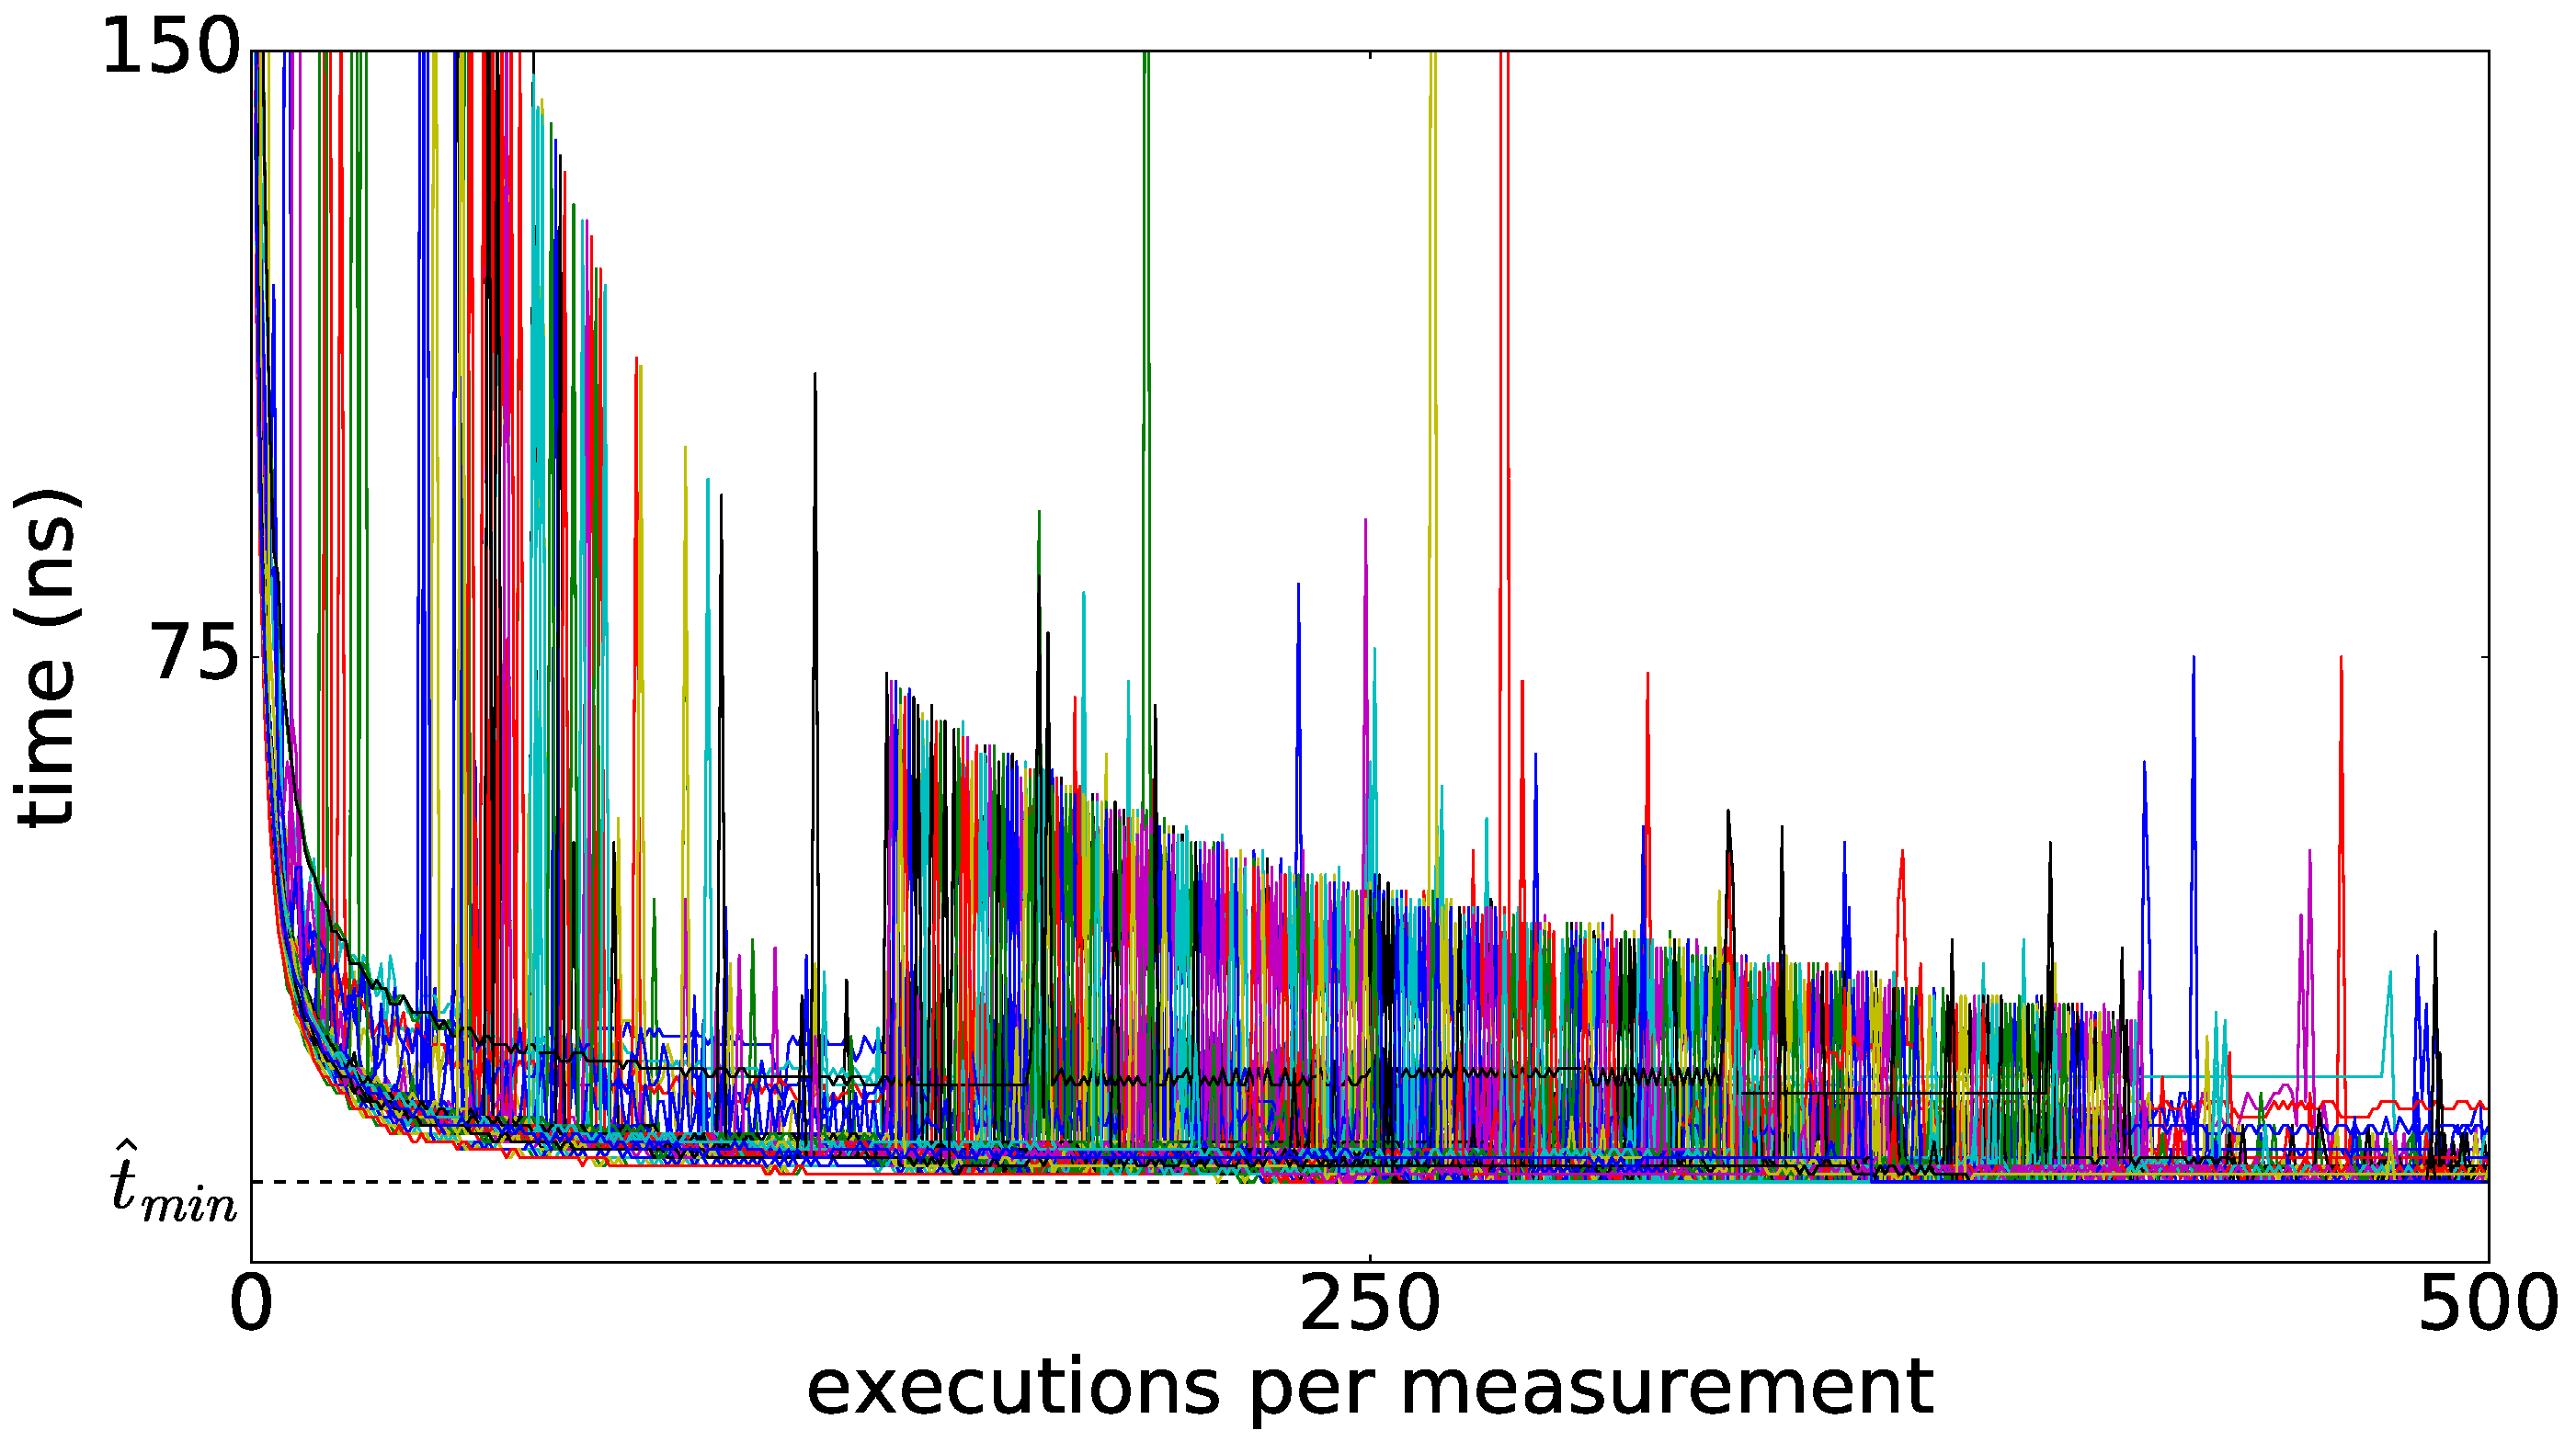
\includegraphics[width=0.45\textwidth]{figures/fig2/linear_scan_branchsum}
\caption{Each curve $i$ plots the coordinates
$\left(1, \frac{T^{\{i\}}_1}{1}\right), \dots,
\left(500, \frac{T^{\{i\}}_{500}}{500}\right)$
gained by executing Algorithm 1 with the same benchmark. Note the relative
smoothness and asymptotic behavior of the cross-curve minima.}
\label{fig:scaling}
\end{figure}

\subsection{Tuning the experiment}

Given $P_0$ (the initial benchmarkable program), $n$ (the number of executions of $P_0$ per
timing measurement), and $\tau_{\textrm{budget}}$ (the user's time budget), an experiment
consists of making several timing measurements $T_1, \dots T_m$ until we have exhausted
$\tau_{\textrm{budget}}$.

Since $P_0$ and $\tau_{\textrm{budget}}$ are fixed by the user, the only parameter we are
free to optimize is $n$. Recalling our model, increasing $n$ can cause $\frac{\epsilon}{n}
\to 0$, thus increasing the accuracy of our estimates $\frac{T_1}{n}, \dots \frac{T_m}{n}$.
However, increasing $n$ also increases the time required to perform a single measurement,
thus decreasing $m$, the number of measurements we can take within the time budget. We can
strike a reasonable balance between maximizing measurement accuracy and maximizing $m$ by
guessing a minimal value of $n$ that renders $\frac{\epsilon}{n} \ll t_{P_0}$. Our
algorithm for guessing this value is as follows:

\begin{algorithm}
    \caption{estimating the optimal $n$ value}
    \KwIn{$P_0$, $\tau_{\textrm{acc}}$, an oracle function $\nu : t \to n$}
    \KwOut{$n$}
    For $i \in \{1, \dots \tau_{\textrm{acc}}\}$, measure the amount of time it takes
    to perform $i$ executions of $P_0$, resulting in a collection of timing measurements
    $T_1, \dots T_{\tau_{\textrm{acc}}}$.

    Estimate $t_{P_0}$ as $\hat{t}_{P_0} = \textrm{min}(\frac{T_1}{1}, \dots \frac{T_{\tau_{\textrm{acc}}}}{\tau_{\textrm{acc}}})$.

    Evaluate $\nu(\hat{t}_{P_0})$ to obtain $n$.
\end{algorithm}

This algorithm only ever needs to be applied once per benchmark, as the optimal value of $n$
for a given $P_0$ can be cached for use in subsequent experiments. Thus, we consider this
algorithm a pre-processing step that does not count against our time budget
$\tau_{\textrm{budget}}$.

\label{sec:minimum}
\subsection{Justifying the minimum estimator}

\begin{figure}
\centering
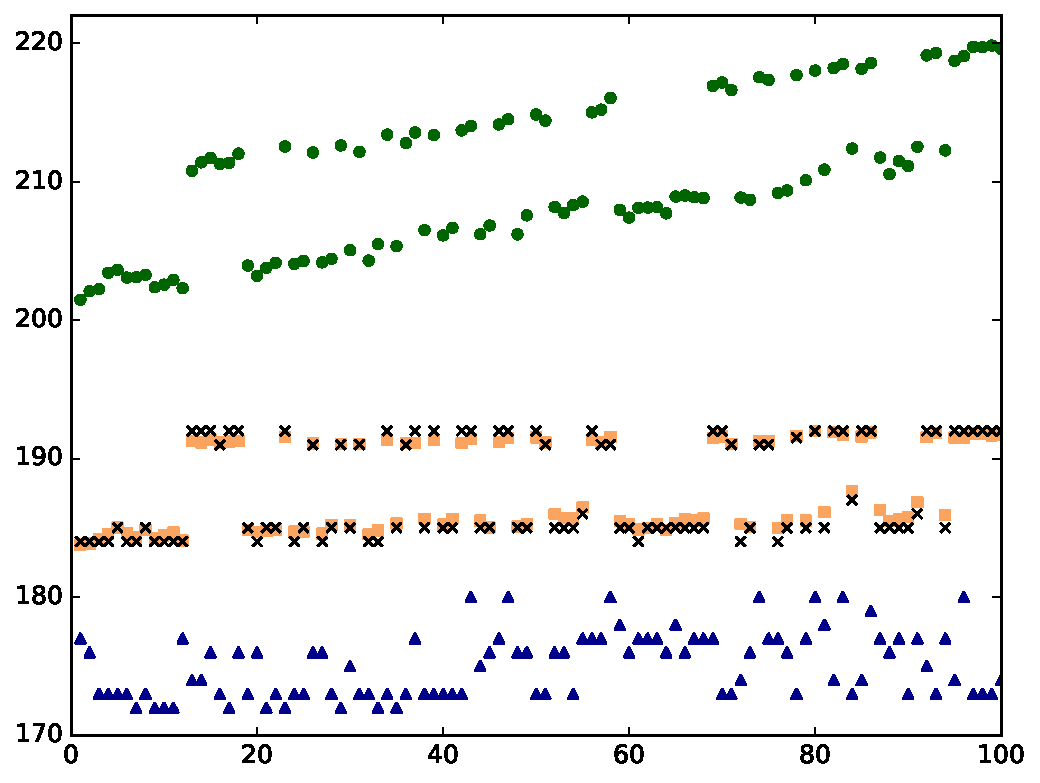
\includegraphics[width=\columnwidth]{figures/fig3/location_estimators_sumindex}
\caption{The behavior of different location parameters across multiple trials of
the \lstinline|sumindex| benchmark: mean (green filled circles), trimmed mean of
the 5th---95th percentiles (brown filled squares), median (black crosses), and
minimum (blue filled triangles).}
\label{fig:locationmeasures}
\end{figure}

% OLD %%%%
% Consider our delay factor term $E = \sum_{i} X_Q^{(i)} \tau^{(i)}$. Given the success
% probabilities $p^{(i)[j]}$ of the Bernoulli variables $x_Q^{(i)[j]}$, there is a minimal
% observable value of $E$ that occurs with nonzero probability. This value, which we'll denote
% $E_{\textrm{min}}$, may not necessarily correspond to $E = 0$, the value attained in the
% theoretical best case where no delay factors trigger during program execution. If at least
% one of the success probabilities is $1$, and the number of instructions in $Q_0$ is $nk$,
% then $\sum_i X_Q^{(i)} \ge nk$ and thus $E = 0$ occurs with zero probability.
% OLD %%%%

In our model, $\textrm{min}(\frac{T_1}{1}, \dots
\frac{T_{\tau_{\textrm{acc}}}}{\tau_{\textrm{acc}}})$ is the best estimator for $t_{P_0}$
because the minimum produces the closest estimate to $t_{P_0}$ attainable from our sample.
Let us justify this claim.

Consider the error term for a given timing measurement $E_m = \frac{\left(\sum_{i} X_Q^{(i)}
\tau^{(i)} + \epsilon \right)_m}{n_m}$, such that $\frac{T_i}{n_i} = t_{P_0} + E_i$. Using
this notation, our justification for using the minimum to estimate $t_{P_0}$ can be written:

\begin{align}
    \hat{t}_{P_0} &= \textrm{min}(\frac{T_1}{1}, \dots \frac{T_{\tau_{\textrm{acc}}}}{\tau_{\textrm{acc}}}) \\ \nonumber
                  &= \textrm{min}(t_{P_0} + E_1, \dots t_{P_0} + E_{\textrm{acc}}) \\ \nonumber
                  &= t_{P_0} + \textrm{min}(E_1, \dots E_{\textrm{acc}}) \\ \nonumber
\end{align}

The minimum thus inherently selects the estimate with the smallest error term.

This interpretation of the minimum is supported by the behavior of the timing estimate curves
plotted in Fig~\ref{fig:scaling}. These curves feature a relatively smooth lower
bound, to which the minimum converges after the region where timer accuracy has a
significant influence on the result. \TODO{say more about this figure?}

Fig~\ref{fig:locationmeasures} provides further justification for the minimum over other
common estimators like the median, mean, or trimmed mean. Recall from
Section~\ref{sec:model} that the $E_i$ terms are sampled from a sum of scaled random
variables following nonidentical Poisson binomial distributions. As such, these terms often
exhibit multimodal behavior. While estimators like the median and trimmed mean are known to
be robust to outliers \TODO{cite}, Fig~\ref{fig:locationmeasures} demonstrates that they
still capture bimodality in the error term distributions. By contrast, we see that the
distribution of the minimum across multiple experimental trials is unimodal, implying that
the minimum is less effected by the bimodally-distributed error terms. \textbf{For our
model, the minimum is a unimodal, robust estimator for the location parameter of a given
benchmark's timing distribution}.

\subsection{Justifying the $n$ range}

It might not be obvious why our heuristic does not test $n > \tau_{\textrm{acc}}$. Recall
that $-\tau_{\textrm{acc}} \le \epsilon \le \tau_{\textrm{acc}}$. For a given value of $n$,
the timer error term in a timing estimate is $\frac{-\tau_{\textrm{acc}}}{n} \le
\frac{\epsilon}{n} \le \frac{\tau_{\textrm{acc}}}{n}$. Thus, when $n = \tau_{\textrm{acc}}$:

\begin{equation}
\frac{-\tau_{\textrm{acc}}}{\tau_{\textrm{acc}}} \le \frac{\epsilon}{\tau_{\textrm{acc}}} \le \frac{\tau_{\textrm{acc}}}{\tau_{\textrm{acc}}} \to -1 \le \frac{\epsilon}{\tau_{\textrm{acc}}} \le 1
\end{equation}

In other words, we do not test $n > \tau_{\textrm{acc}}$ since the error at $n \ge
\tau_{\textrm{acc}}$ is contrained to timer precision.

\subsection{The oracle function}

\begin{figure}
\centering
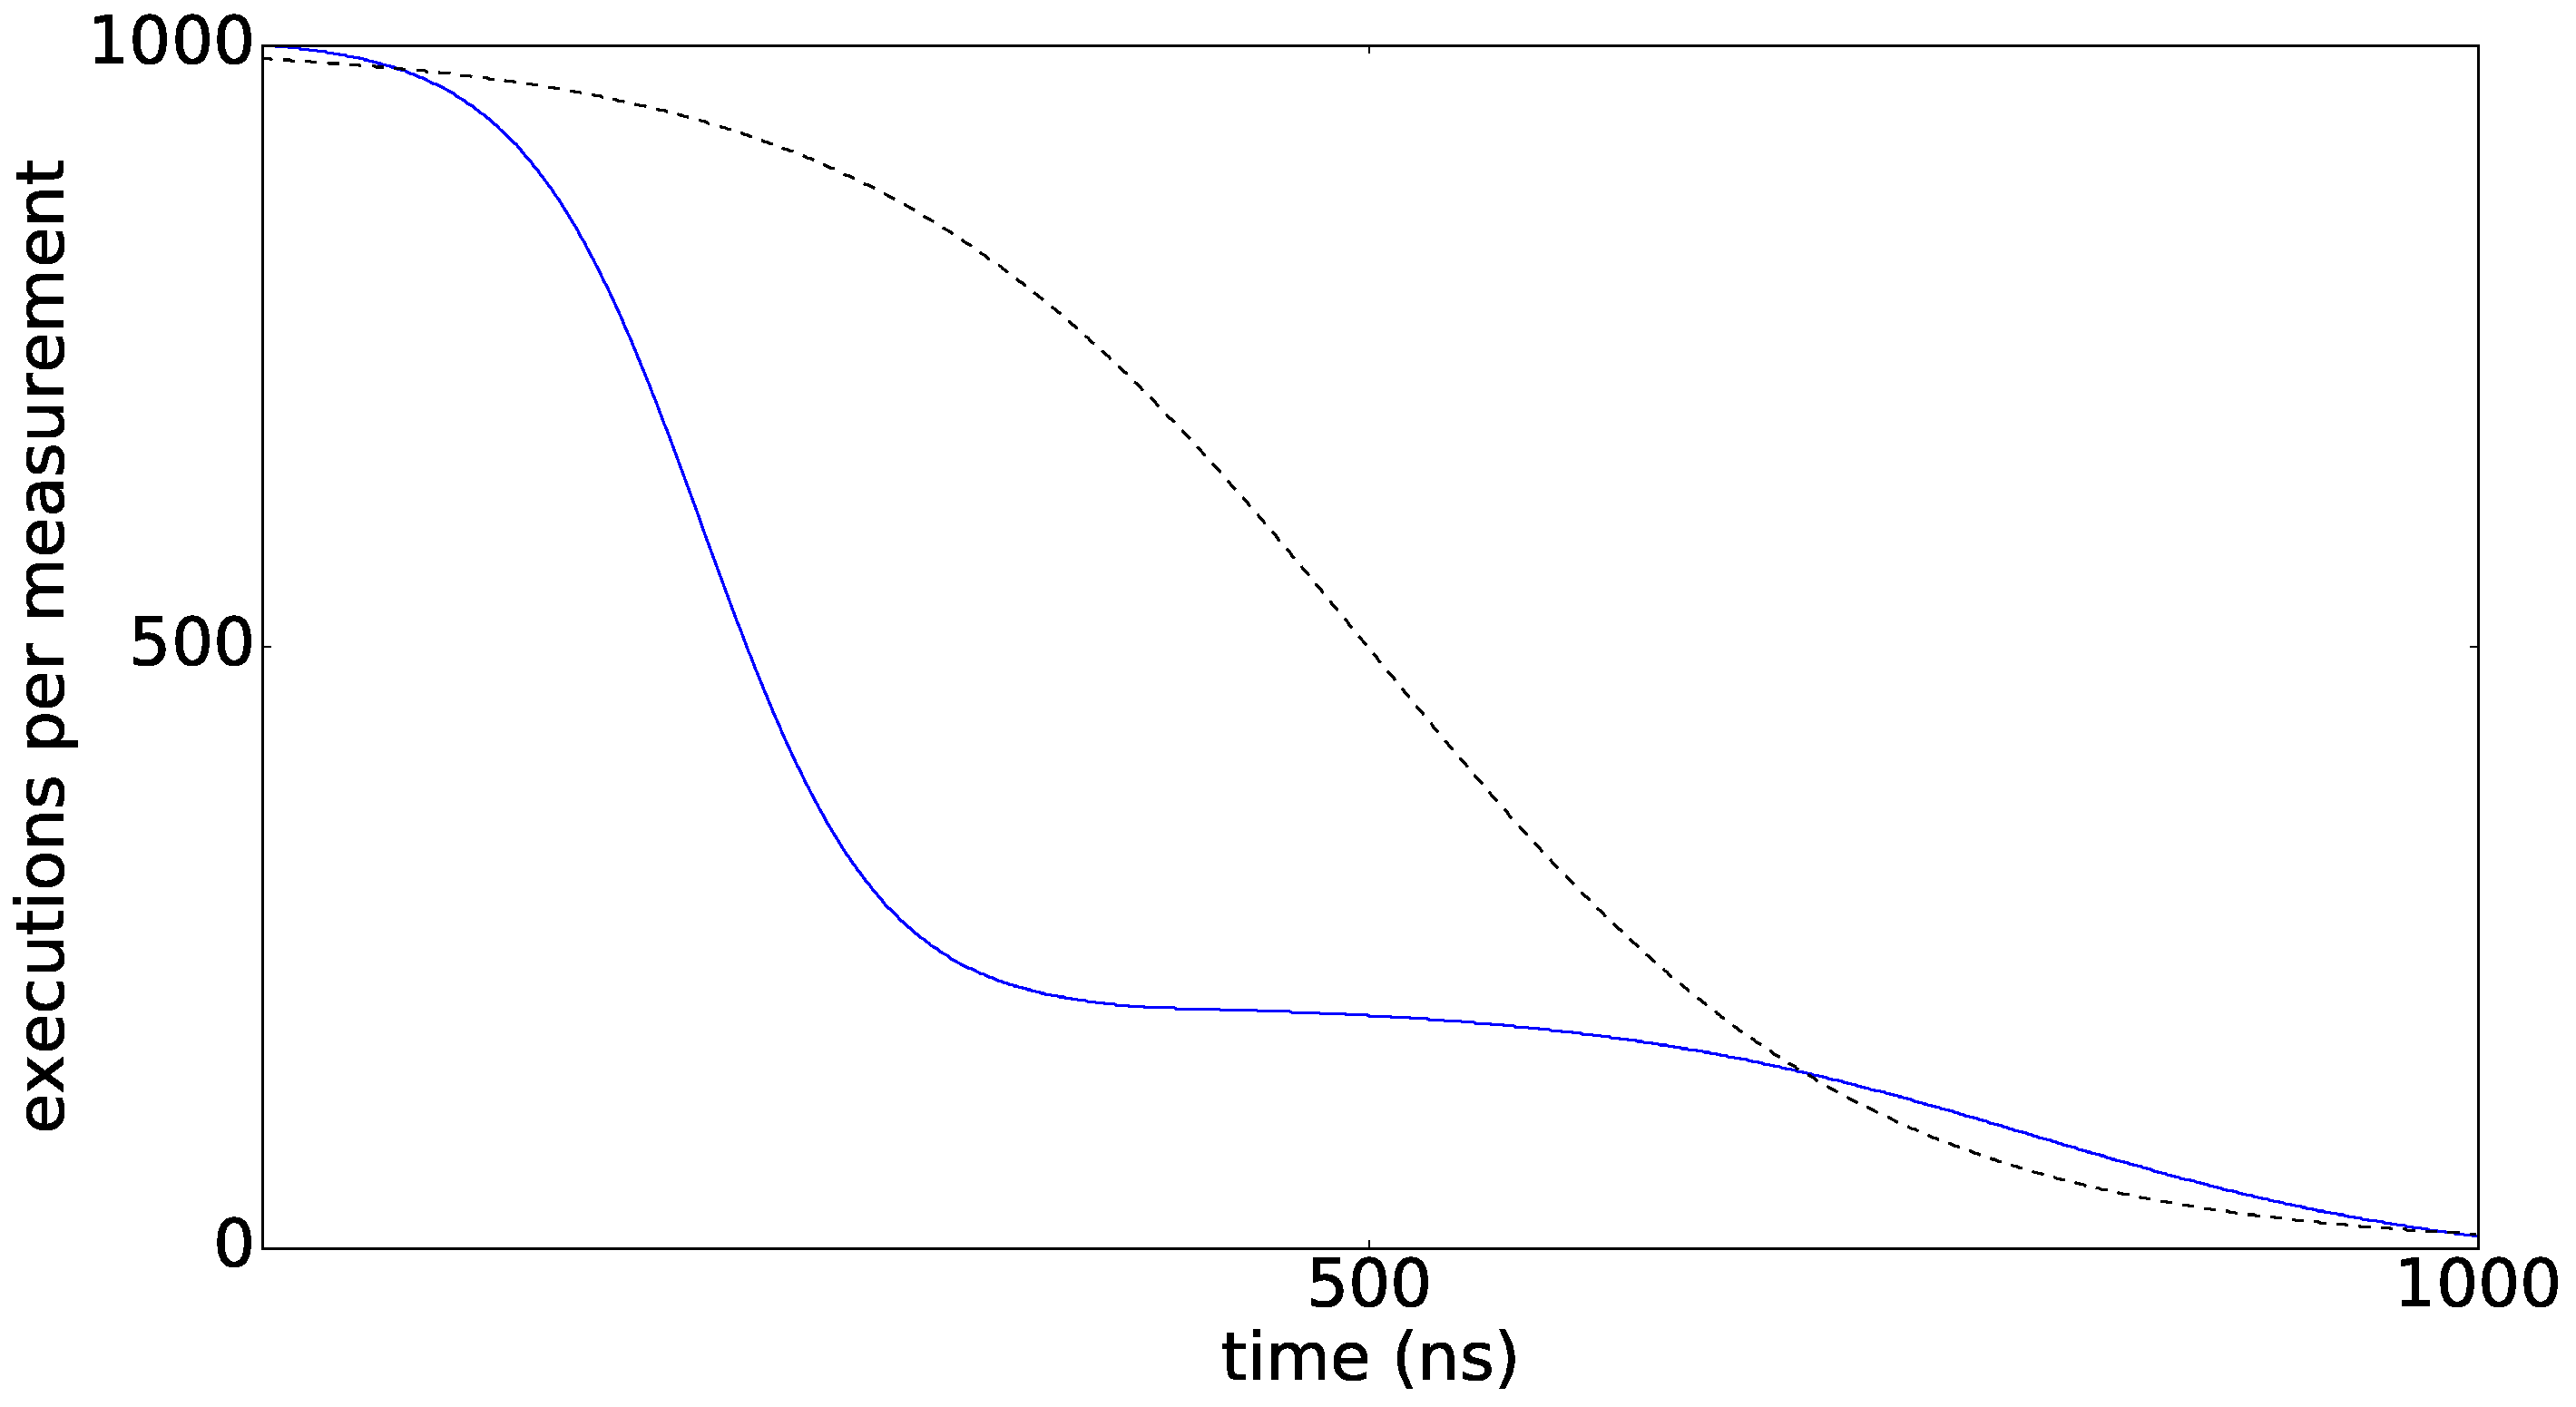
\includegraphics[width=0.45\textwidth]{figures/fig5/oracle}
\caption{Two possible curves for $\nu(t)$ at $\tau_{\textrm{acc}} \approx 1000 \textrm{ns}$.
The solid blue curve is an example of an empirically-tuned lookup table, while the dotted
black curve is $Y(t)$ from Eq~\ref{eq:14} with parameters $a = 0.009$ and $b = 0.5$.}
\label{fig:scaling}
\end{figure}

Our heuristic takes as input an oracle function $\nu(t)$ that maps expected runtimes to an
optimal number of executions per measurement. While Algorithm 1 does not directly describe
$\nu(t)$, appropriate choices for this function should have the following properties:

\begin{itemize}
    \item $\nu(t)$ has a discrete range $n \in \{1, \dots \tau_{\textrm{acc}}\}$
    \item $\nu(t)$ is monotonically decreasing
    \item $\frac{d\nu}{dt}|_{t \approx 1} \approx 0$
    \item $\frac{d\nu}{dt}|_{t \approx \tau_{\textrm{acc}}} \approx 0$
    \item $\nu(1) \approx \tau_{\textrm{acc}}$
    \item $\nu(t \ge \tau_{\textrm{acc}}) \approx 1$
\end{itemize}

Some of the above properties require further motivation. First, $\nu(t)$ should be
monotonically decreasing because benchmarks with larger runtimes will require smaller $n$,
and vice versa. Second, $\nu(t)$ should be relatively flat for small $t$ because variations
in the error term between timing estimates can be large compared to the actual runtime of
fast benchmarks.

A useful realization of $\nu(t)$ is a special version of the generalized logistic function
that can be tuned to achieve the above properties. For our purposes, we can express this
function as

\begin{equation}
    Y(t) = \floor*{1 + \frac{\tau_{\textrm{acc}} - 1}{1 + e^{a * (t - b*\tau_{\textrm{acc}})}}}
\end{equation}

where reasonable values of $a$ and $b$ are approximately $0.005 < a < 0.02$ and $0.4 < b <
0.6$. In practice, we have found that more optimal results can be achieved by first
approximating $Y(t)$ with a lookup table, then modifying the lookup table based on empirical
observations. This was accomplished by examining many benchmarks with a variety of known
runtimes at different time scales, seeking for each runtime the smallest $n$ value at which
the minimum estimate appears to converge to a lower bound (e.g. around $n = 250$ for the
benchmark in Fig~\ref{fig:scaling}). Fig~\ref{fig:oracle} plots both Eq~\ref{eq:14} and an
empirically obtained lookup table as potential oracle functions.

%%%%%%%%%%%%%%%%%%%%%%%%%%%%%%%%%%%%%%%%%%%%%%%%%%%%%%%%%%%%%%%%%%%%%%%%%%%%%%%%%%%%%%%%%%%%
\label{sec:hypotesting}
\section{Barriers to statistical tests of benchmark timings}

The chief problem we have encountered doing real-world performance testing is not detecting
changes in $\hat{t}_{P_0}$ between two versions of the same program, but is rather
automatically deciding if the change is \textit{statistically significant}.

Commonly used statistical tests start with the assumption that samples are idependent and
identically distributed (i.i.d). Our model does not enforce this to be the case


Many statistical tests rely on two assumptions:
In this section, we will highlight the properties of our model that make designing
statistical tests difficult, and demonstrate how these properties can




formulate a nonparametric hypothesis test and effect size threshold that enables the
automatic determination of a given performance change's statistical significance.

To accomplish this, we formulate our test around a falsifiable null hypothesis. Given a
program $P_0$ and another program $R_0$, our null hypothesis is that the runtimes of
the two programs are equal in the absence of error:

\begin{equation}
    H_0: t_{P_0} = t_{R_0}
\end{equation}

In order to evaluate this claim, we can write out our hypothesis test in terms of a
parameter $z$ and it's value under the null hypothesis $z_0$. As is common when the null
hypothesis is an equality\TODO{cite}, we will choose our parameter to be the ratio
of the two values we are comparing:

\begin{align}
    z   &= \frac{t_{P_0}}{t_{R_0}} \\
    z_{H_0} &= 1
\end{align}

The next step is to derive a \textit{test statistic} that serves as an \textit{estimator}
for $z$. We can accomplish this by referring to the timing estimators established in
Section~\ref{sec:minimum}:

\begin{align}
    \hat{z} = \frac{\hat{t}_{P_0}}{\hat{t}_{R_0}} = \frac{\textrm{min}(T_P)}{\textrm{min}(T_R)}
\end{align}

This estimator can be applied to experimentally observed timing measurements to produce an
estimate (by convention, also referred to as $\hat{z}$).

\begin{equation}
    \hat{z} = \frac{\hat{t}_{P_0}}{\hat{t}_{R_0}} = \frac{\textrm{min}((T_1, \dots T_{m_P})_{P_0})}{\textrm{min}((T_1, \dots T_{m_R})_{R_0})}
\end{equation}

While the parameter $z$ is fixed with respect to $P_0$ and $R_0$, its estimator $\hat{z}$ is
a random variable that depends on the error terms $E_R$ and $E_P$. Thus, $\hat{z}$'s
distribution depends on the distribution followed by $E_R$ and $E_P$. As defined in
Section~\ref{sec:model}, the delay instructions that produce these distributions are program
dependent. This makes it difficult to derive $\hat{z}$ distribution in a general case. Since
analytically deriving of the distribution for every pair of input programs is untenable, we
can leverage existing resampling methods to perform nonparametric hypothesis testing.

\subsection{Choosing a resampling method}

One of the most commonly used nonparametric statistical techniques is the \textit{bootstrap
resampling method}. In this method, a guess is formed for the estimator's distribution by
repeatedly applying the estimator to randomly selected resamples of the original data. The
yielded distribution can then be used to perform a standard one-tailed or two-tailed
hypothesis test.

In this section, we'll discuss the various ways in which the standard bootstrap fails,
and argue that a bootstrap variant known as the \textit{subsampling method} is the
appropriate technique for our use case.

The standard bootstrap dictates that the resample size equals the original sample size,
and that the original data is uniformly resampled with replacement \footnote{\TODO{explain
replacement}}. This strategy is problematic in two respects:

\begin{enumerate}
    \item It produces degenerate distributions for extrema estimators such as the minimum \TODO{cite}.
    \item It assumes the original data is i.i.d. The resampled data does not preserve dependency
    structures that might be present in the original data \TODO{cite}.
\end{enumerate}

To solve the first problem, it is sufficient to select a resample size $m$ that is smaller
than the original sample size $n$, with the restriction that one's method for calculating
$m$ must obey $m \to \infty$ and $\frac{m}{n} \to 0$ as $n \to \infty$
\footnote{\TODO{mention data-dependent methods of calculating optimal $m$}}. This variant of
the bootstrap is known as \textit{m-out-of-n bootstrap}.

To solve the second problem, we must modify our resampling strategy such that resampled data
replicates potential autocorrelations in the original data. This can be accomplished by
performing what is known as the \textit{block bootstrap}, where the resample population is
taken to be blocks of consecutive measurements rather than individual measurements. The
order of magnitude of the block size $b$ determines the success and convergence rate of the
block bootstrap. An $n$-dependent calculation of $b$ generally must follow the same
restriction as the $n$-dependent calculation of $m$ from the m-out-of-n bootstrap, namely
that $b \to \infty$ and $\frac{b}{n} \to 0$ as $n \to \infty$.

While each of these variants solves one of our two problems, neither approach solves both.
Fortunately, these techniques are not mutually exclusive - one can perform a block bootstrap
in which the resample size is smaller than the original sample size. The case in which a
block bootstrap is performed with a resample size of one is known as \textit{subsampling},
and has been proven to work for the estimation of extrema distributions of autocorrelated
data \TODO{cite}.

At this point, the reader would be wise to ask why the subsampling method is not more
popular than the bootstrap, given that it succeeds under fewer restrictions. The answer
is that the success of the subsampling method is extremely susceptible to choices in



 \footnote{The reader might wonder why the standard bootstrap is so
popular, given that the subsampling method succeeds under fewer restrictions on the
distribution being estimated. Firstly, it was not until 1995 that Bertail et. al. proved
that subsampling was tractable for estimators with unknown rates of convergence \TODO{cite}.
Secondly, data-dependent methods for rigorously choosing the subsample size $b$ can be
prohibitively computationally intensive (depending on which method is used), as it can
require repeating the entire resampling process at multiple $b$ values \TODO{cite}.}

\subsection{Implementation in Julia}

%%%%%%%%%%%%%%%%%%%%%%%%%%%%%%%%%%%%%%%%%%%%%%%%%%%%%%%%%%%%%%%%%%%%%%%%%%%%%%%%%%%%%%%%%%%%
\label{sec:julia}
\section{Results on Julia Benchmarks}

To test our approach, we wrote a small set of mock benchmarks, each of which has additional
``fast'' and ``slow'' implementations:

\begin{itemize}
    \item The \lstinline|sumindex(a, inds)| benchmark sums over all \lstinline|a[i]| for all \lstinline|i| in \lstinline|inds|. The normal version uses the array \lstinline|[1, 2, ..., length(a)]| for \lstinline|inds|. This test stresses memory layout via element retrieval.
    \begin{itemize}
        \item \lstinline|sumindex_fast(a)| replaces the normal version's \lstinline|inds| array with a range \lstinline|1:length(a)|.
        \item \lstinline|sumindex_slow(a)| reverses the normal version's \lstinline|inds| array, instead summing over the indices \lstinline|[length(a), ..., 2, 1]|.
    \end{itemize}
    \item The \lstinline|pushall!(a, b)| benchmark pushes elements from \lstinline|b| into \lstinline|a| one by one, additionally generating a random number at each iteration (the random number does not affect the output). This test stresses both random number generation and periodic reallocation that occurs as part of Julia's dynamic array resizing algorithm.
    \begin{itemize}
        \item \lstinline|pushall_fast!(a, b)| removes the extraneous random number generation at each iteration.
        \item \lstinline|pushall_slow!(a, b)| generates an additional random number at each iteration.
    \end{itemize}
    \item The \lstinline|branchsum(n)| benchmark loops from \lstinline|1| to \lstinline|n|. If the loop variable is even, a counter is decremented. Otherwise, an inner loop is triggered which runs from \lstinline|1| to \lstinline|n|, in which another parity test is performed on the inner loop variable to determine whether to increment or decrement the counter. This test stresses periodically costly branching within loop iterations.
    \begin{itemize}
        \item \lstinline|branchsum_fast(n)| lifts the first parity test outside the loop, and uses it as a base case for recursive calls that are triggered within the loop (calls to \lstinline|branchsum_fast(i)| where \lstinline|i| is the loop variable).
        \item \lstinline|branchsum_slow(n)| is structured similarly to \lstinline|branchsum_fast(n)|, but uses full \lstinline|if|/\lstinline|else| statements whose bodies are the summation expressions, instead of the ternary operators used in \lstinline|branchsum_fast(n)|, whose bodies are only the integers to be summed.
    \end{itemize}
    \item The \lstinline|manyallocs(n)| allocates an array of \lstinline|n| elements, where each element is itself an array. The inner array length is determined by a random number from \lstinline|1| to \lstinline|n|, which is regenerated when each new array is constructed. However, the random number generator is reseeded before each generation so that the program is deterministic. This test stresses random number generation and frequent allocations of unpredictable size, even though in reality the lengths are deterministic and uniform.
    \begin{itemize}
        \item \lstinline|manyallocs_fast(n)| only generates the inner array length once, before all arrays are constructed.
        \item \lstinline|manyallocs_slow(n)| constructs each inner array by dynamically resizing it rather than preallocating memory for it, and additionally performs an unnecessary copy of each inner array.
    \end{itemize}
\end{itemize}

For every benchmark implementation, 100 experimental trials were performed. Each trial
consisted of 10,000 timing measurements, where the number of benchmark executions per
measurement was predetermined by the procedure given in \ref{sec:tuningprotocol}.

The artificial regressions and improvements introduced by the ``fast'' and ``slow'' versions
of these benchmarks allow us to empirically observe false negative (incorrect non-rejection
of the null hypothesis) and false positive (incorrect rejection of the null hypothesis)
rates for our regression detection test. Three separate tests were performed in order to
derive these estimates:

\begin{enumerate}
\item We tested our detection algorithm against every pairwise combination of trials for each
benchmark's control, fast, and slow implementations. This corresponds to 90,000 tests per
benchmark (10,000 pairwise trial combinations times 9 pairwise implementation combinations).
% No false negatives or positives were detected.
\item We tested our detection algorithm against 20 million random pairs of trials, where our
population contained all trials of all benchmarks. % Again, no false negatives or positives
% were detected.
\item We tested our detection algorithm on $\sim$600 benchmarks from the Julia's core benchmark
suite, which is implemented in the BaseBenchmarks.jl package. We selected only the
benchmarks for which we had the time to collect at least 10,000 timing measurements, which
are also the benchmarks in the relevant time scale of the tens of microseconds or lower
(microbenchmarks). % The false positive rate was 0.056.
\end{enumerate}

% For each test, the threshold of rejection was 0.01 (1\%), the resample size was 5, and the
% original populations were resampled 1000 times.

\begin{figure}[!t]
\centering
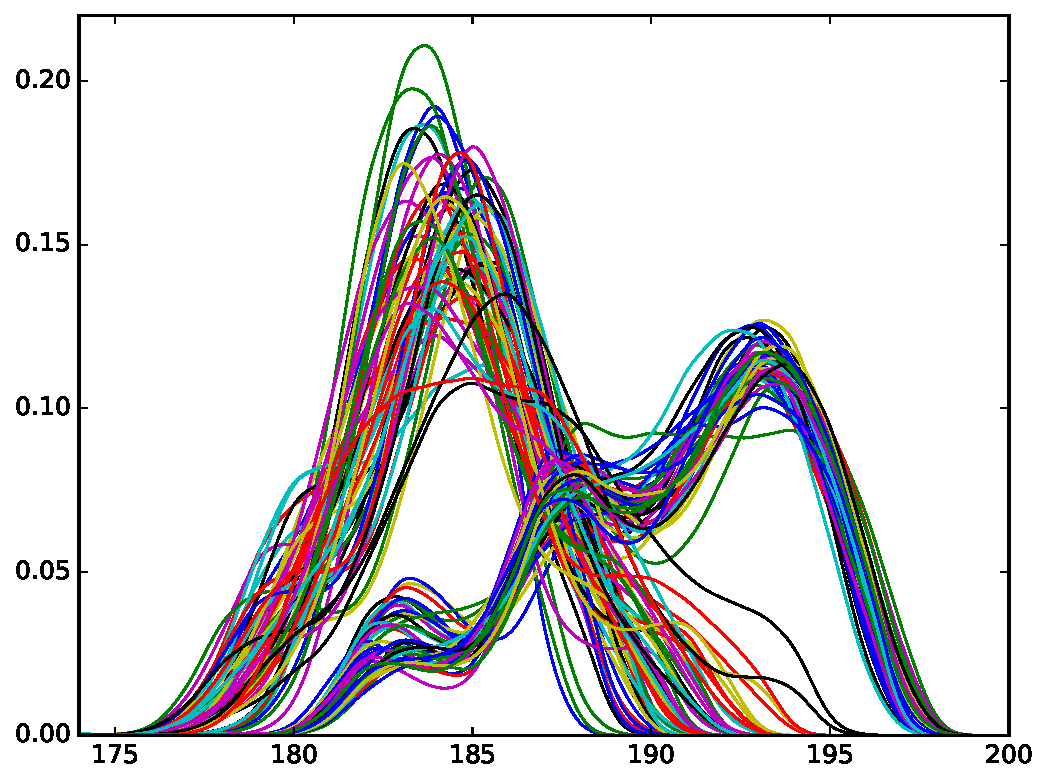
\includegraphics[width=\columnwidth]{figures/fig4/kde_pdf_sumindex}
\caption{Kernel density estimates (KDEs) of the probability density function of the
\lstinline|sumindex| benchmark. Each line is a single KDE constructed from an
individual trial of 10,000 timing measurements. Each trial was performed}
\label{fig:pdfsumindex}
\end{figure}

%%%%%%%%%%%%%%%%%%%%%%%%%%%%%%%%%%%%%%%%%%%%%%%%%%%%%%%%%%%%%%%%%%%%%%%%%%%%%%%%%%%%%%%%%%%%

\label{sec:conclusion}
\section{Conclusion}

%%%%%%%%%%%%%%%%%%%%%%%%%%%%%%%%%%%%%%%%%%%%%%%%%%%%%%%%%%%%%%%%%%%%%%%%%%%%%%%%%%%%%%%%%%%%
\label{sec:acknowledgement}
\section*{Acknowledgment}

We thank the many Julia developers, in particular Andreas Noack and Steven G.
Johnson of MIT, for many insightful discussions.
This research was supported (in part) by the U.S. Army Research Office under
contract W911NF-13-D-0001.

%%%%%%%%%%%%%%%%%%%%%%%%%%%%%%%%%%%%%%%%%%%%%%%%%%%%%%%%%%%%%%%%%%%%%%%%%%%%%%%%%%%%%%%%%%%%
\bibliography{biblio}
\bibliographystyle{IEEEtran}

% that's all folks
\end{document}
\grid
